\documentclass[12pt,a4paper,fleqn]{article}
\usepackage{rmpackages}																% usual packages
\usepackage{rmtemplate}																% graphic charter
\usepackage{rmexocptce}																% for DS with cptce eval

%\cfoot{} 													% if no page number is needed
%\renewcommand\arraystretch{1.5}		% stretch table line height

\begin{document}

\section*{Version 1}

\begin{center}
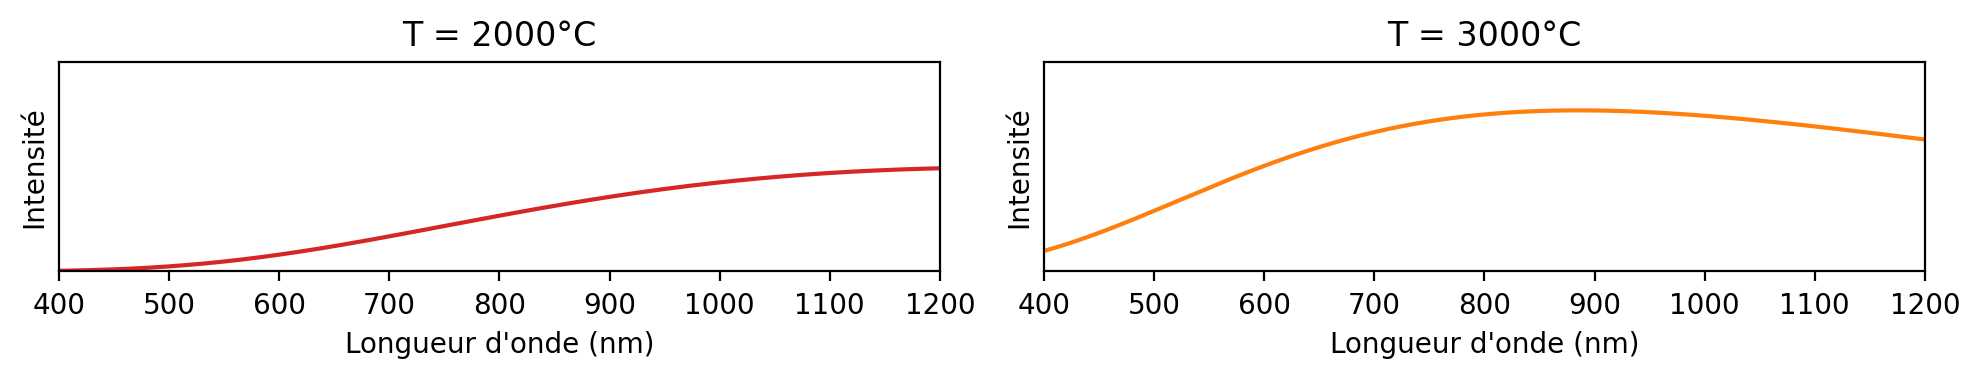
\includegraphics[width=\linewidth]{images/spectrum_black_body_curve3273K.png}
\end{center}

\begin{center}
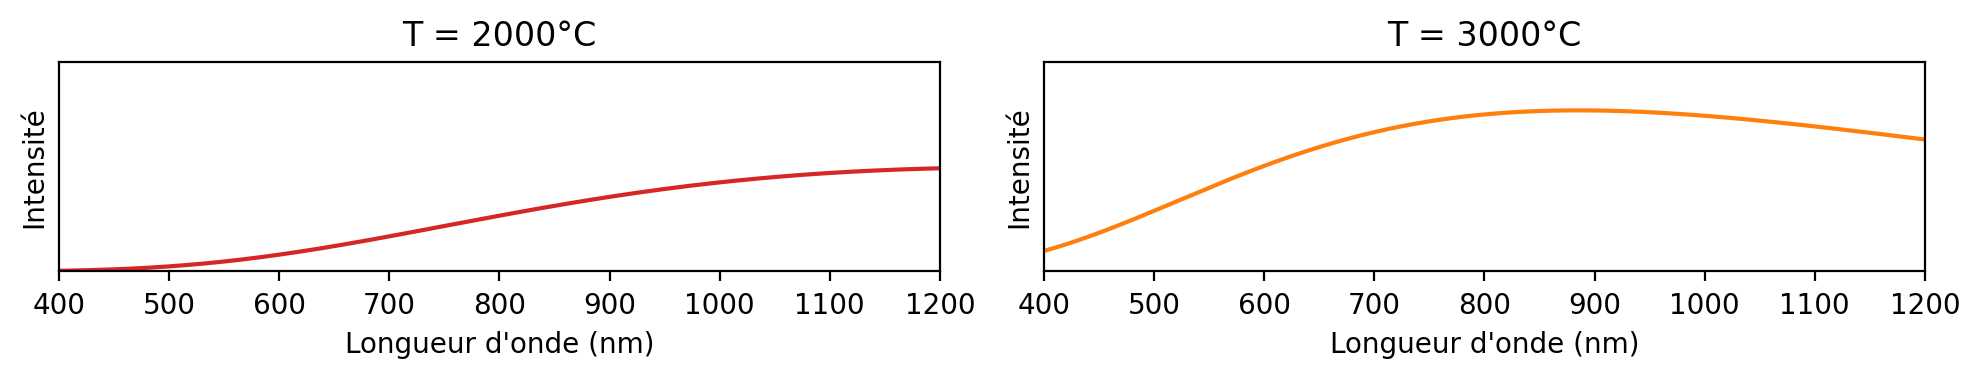
\includegraphics[width=\linewidth]{images/spectrum_black_body_curve3273K.png}
\end{center}

\begin{center}
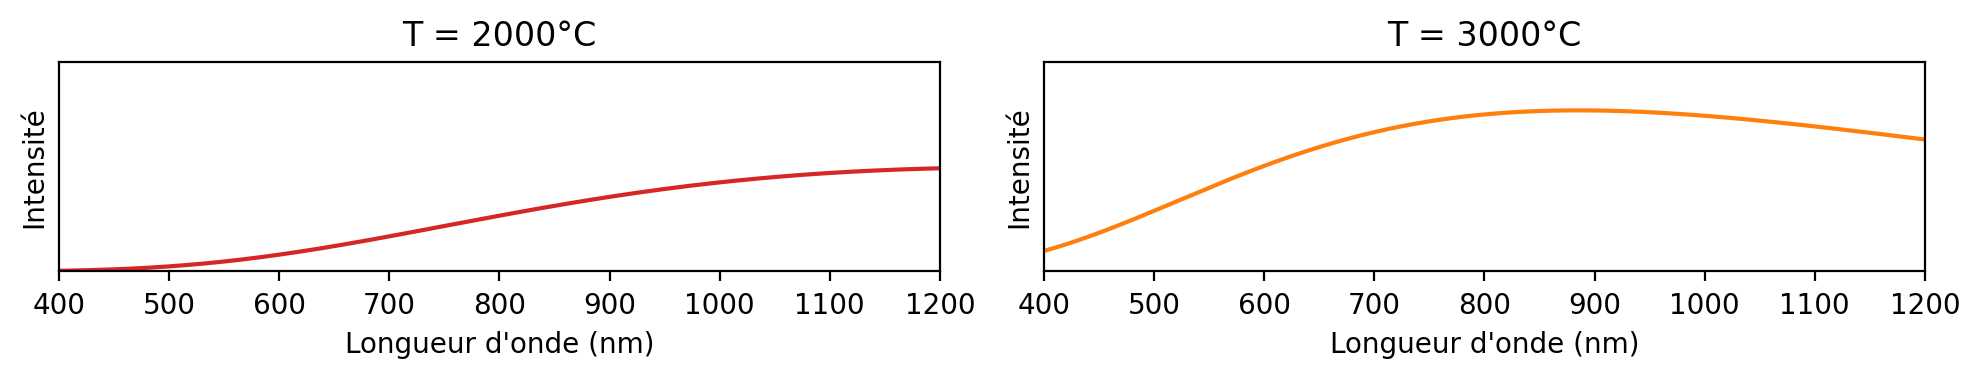
\includegraphics[width=\linewidth]{images/spectrum_black_body_curve3273K.png}
\end{center}

\begin{center}
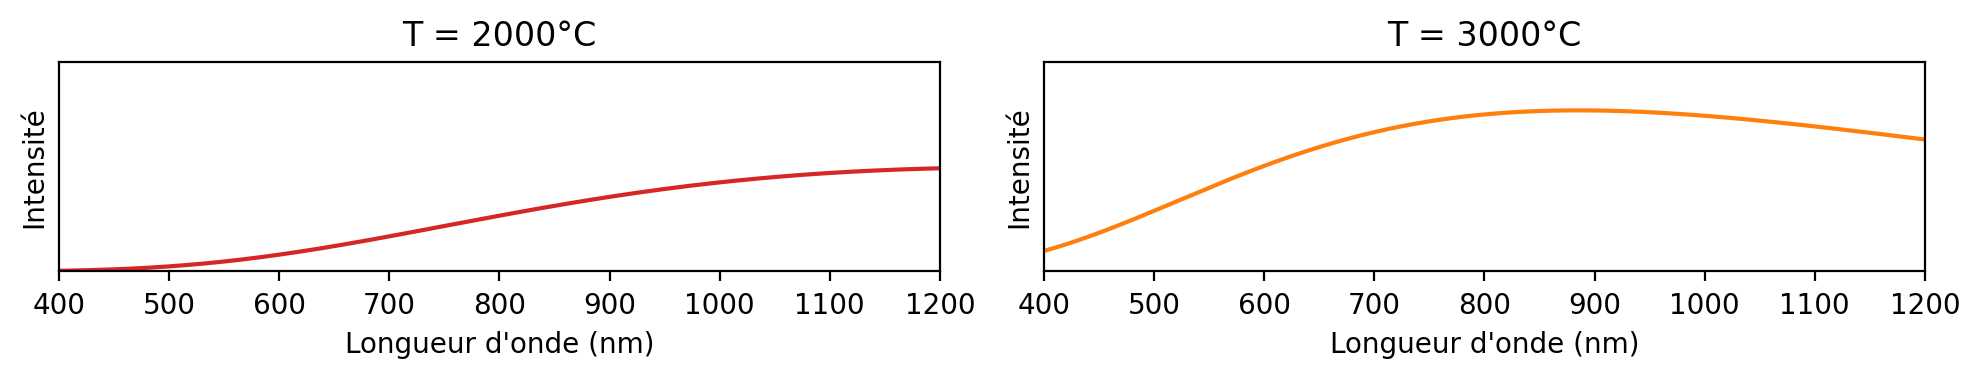
\includegraphics[width=\linewidth]{images/spectrum_black_body_curve3273K.png}
\end{center}

\begin{center}
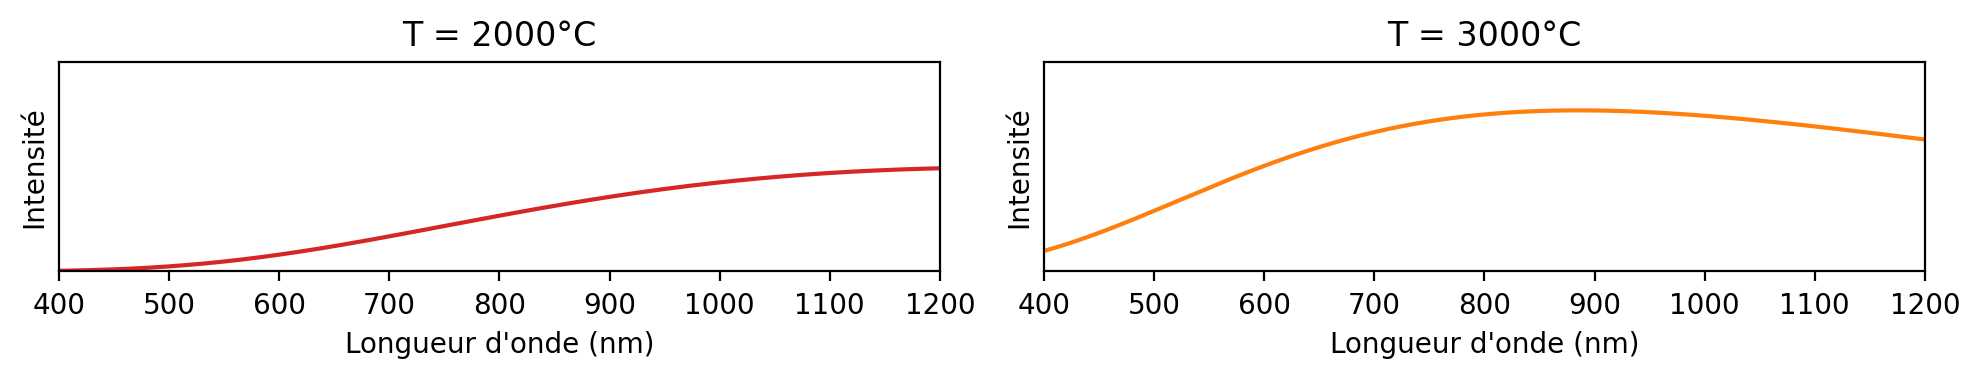
\includegraphics[width=\linewidth]{images/spectrum_black_body_curve3273K.png}
\end{center}

\begin{center}
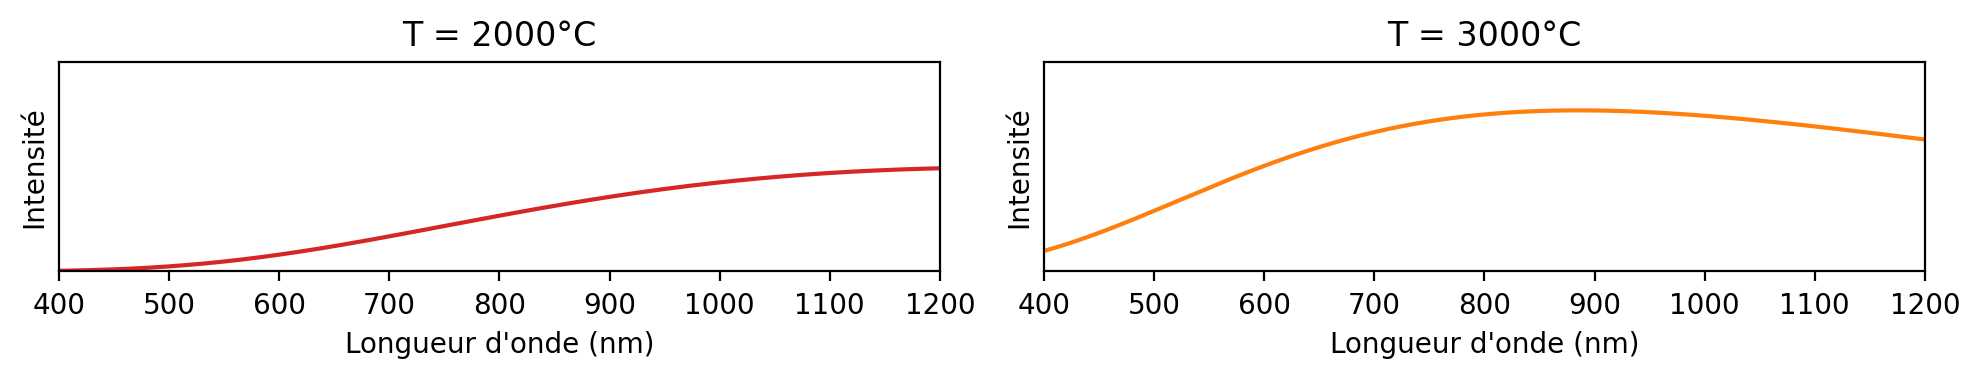
\includegraphics[width=\linewidth]{images/spectrum_black_body_curve3273K.png}
\end{center}

\newpage
\section*{Version 2}

\begin{center}
\begin{multicols}{2}

\includegraphics[width=\linewidth]{images/spectrum_black_body_temp2500K.png}


\includegraphics[width=\linewidth]{images/spectrum_black_body_temp4000K.png}
\end{multicols}
La flèche indique la radiation émise avec le maximum d'intensité.
\end{center}

\begin{center}
\begin{multicols}{2}

\includegraphics[width=\linewidth]{images/spectrum_black_body_temp2500K.png}


\includegraphics[width=\linewidth]{images/spectrum_black_body_temp4000K.png}
\end{multicols}
La flèche indique la radiation émise avec le maximum d'intensité.
\end{center}

\begin{center}
\begin{multicols}{2}

\includegraphics[width=\linewidth]{images/spectrum_black_body_temp2500K.png}


\includegraphics[width=\linewidth]{images/spectrum_black_body_temp4000K.png}
\end{multicols}
La flèche indique la radiation émise avec le maximum d'intensité.
\end{center}

\begin{center}
\begin{multicols}{2}

\includegraphics[width=\linewidth]{images/spectrum_black_body_temp2500K.png}


\includegraphics[width=\linewidth]{images/spectrum_black_body_temp4000K.png}
\end{multicols}
La flèche indique la radiation émise avec le maximum d'intensité.
\end{center}

\begin{center}
\begin{multicols}{2}

\includegraphics[width=\linewidth]{images/spectrum_black_body_temp2500K.png}


\includegraphics[width=\linewidth]{images/spectrum_black_body_temp4000K.png}
\end{multicols}
La flèche indique la radiation émise avec le maximum d'intensité.
\end{center}

\begin{center}
\begin{multicols}{2}

\includegraphics[width=\linewidth]{images/spectrum_black_body_temp2500K.png}


\includegraphics[width=\linewidth]{images/spectrum_black_body_temp4000K.png}
\end{multicols}
La flèche indique la radiation émise avec le maximum d'intensité.
\end{center}


\end{document}